\section{Justificaci\'on del Proyecto}\label{sec:justificacion}

\begin{figure}[H]
  \centering
  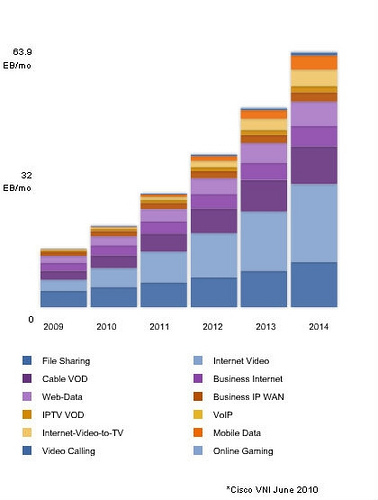
\includegraphics[width=12cm]{Imagenes/aumento_bw.png}
  \caption{Tendencia en el aumento del ancho de banda a nivel mundial
    según un estudio de Cisco de 2013.}
  \label{fig:aumento_bw}
\end{figure}

A medida que crece el requerimiento de ancho de banda de los usuarios
en internet, las empresas proveedoras del servicio deben utilizar más
y más tecnologías extensibles y flexibles que posibiliten este
proceso.

Como muestra la figura \ref{fig:aumento_bw}, el crecimiento de ancho
de banda a nivel global está en aumento constante. Se espera que este
crecimiento no se detenga nunca, ya que a medida que el ser humano
tiene más y más velocidad, mayores son sus necesidades y exigencias de
la tecnología.

\emph{DWDM} es una tecnología en esencia modular y escalable. Todos
los proveedores de esta tecnología ofrecen actualizaciones en forma de
módulos para poder reemplazar los equipos viejos con generaciones
nuevas o bien para poder expandir el soporte de las tecnologías
tradicionales a más tendidos.

La incursión de los \emph{OADM} hacia un sistema programable con
variedad de filtros integrado y con manejo de eventos, como lo es
\emph{WSS}, ha significado que la flexibilidad de \emph{DWDM} es mayor
que nunca. Por otro lado, los precios de estos dispositivos han
disminuido de forma considerable los últimos años, haciéndose
populares y soportados globalmente.

Las redes fotónicas ``oscuras'', es decir, sin ningún tipo de
multiplexación o control de las señales al momento de introducirlas en
la fibra, no son adecuadas para montar redes modernas que requieran
grandes anchos de banda. Sobre todo entre datacenters, los cuales son
lugares donde el volumen y la importancia de los datos que fluyen
hacia y desde estos nodos deben cumplir con tener un acceso cada vez
más rápido y por parte de más usuarios.

Algunos de los servicios más pintorescos que permiten implementar los
data centers en el mundo son los que se muestran en la figura
\ref{fig:servicios}.

\begin{figure}[H]
  \centering
  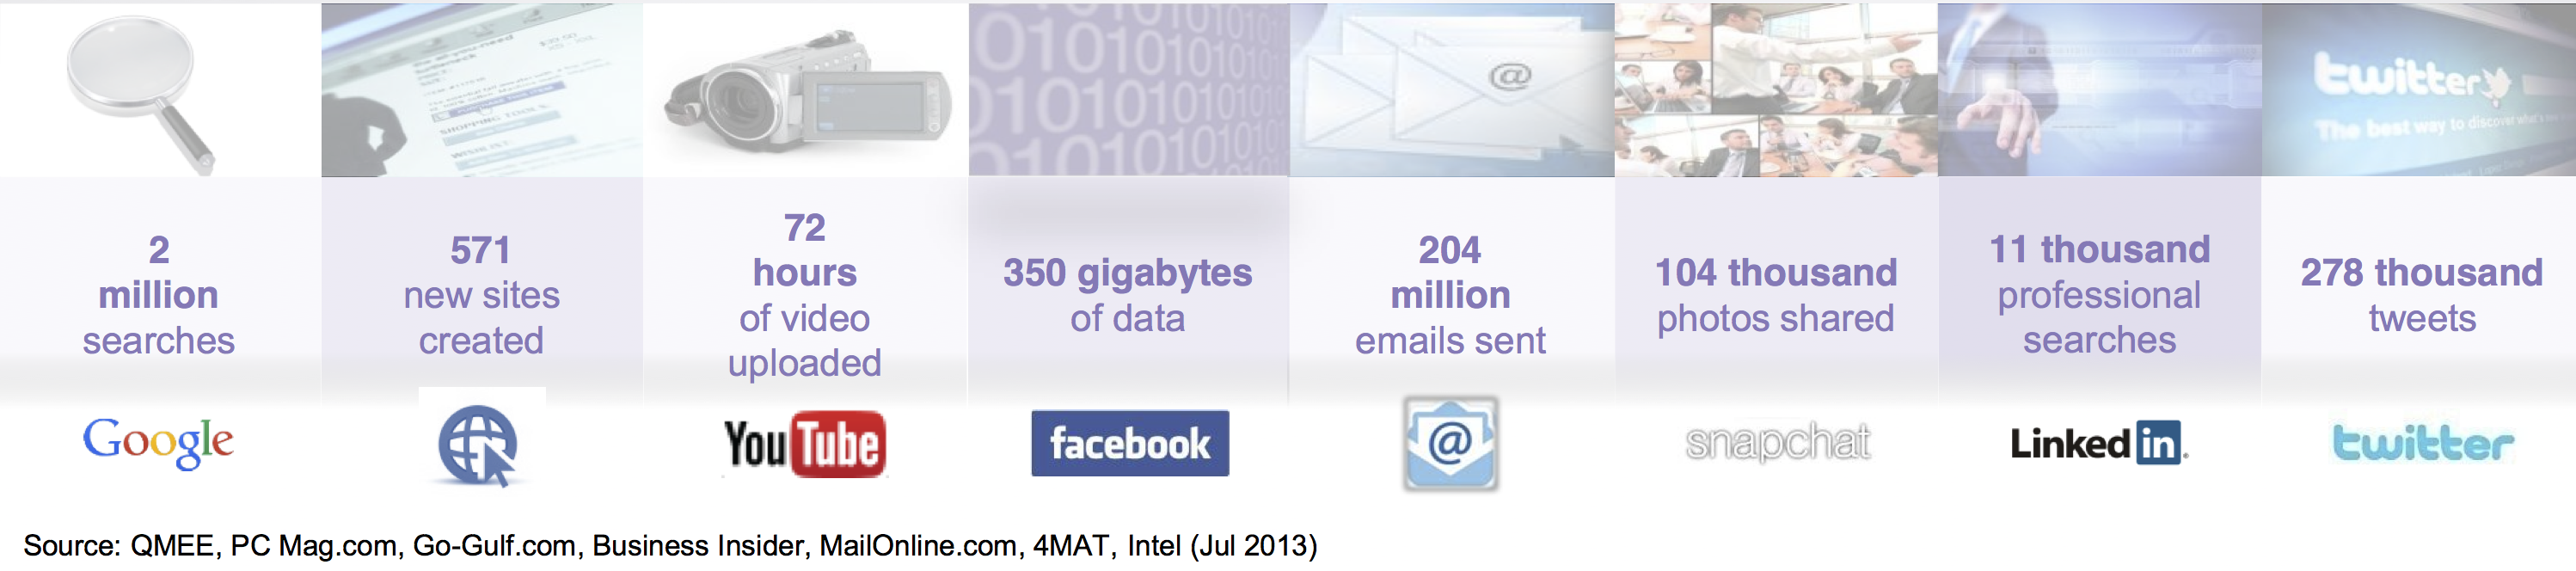
\includegraphics[width=15cm]{Imagenes/servicios.png}
  \caption{Servicios en los que participan data centers que ocupan una
    muy alta y creciente cantidad de capacidad instalada en las
    redes. Datos de julio de 2013 provenientes de: QMEE, PC Mag.com,
    Go-Gulf.com, Business Insider, MailOnline.com, 4MAT e Intel.}
  \label{fig:servicios}
\end{figure}

En definitiva, el avance de la tecnología y la disminución de precios
que han experimentado son los factores más importantes que permiten
justificar el proyecto. 
